\newpage
\section{Visualisierung mit Unreal Engine}
Ein digitaler Nachbau der Gegebenheiten der Aufgabenstellung bietet verschiedene Vorteile. Dazu gehört es, Probleme können bereits zu erkennen, bevor physische Produkte bestellt werden müssen, sowie in dem Fall die potentielle Beschaffung von Trainingsdaten für die Bilderkennung. Unreal Engine, ursprünglich eine 3D Spiele-Engine, die mittlerweise viele weitere Einsatzgebiete hat, erlaubt die einfache Umsetzung einer virtuellen Umgebung, sowie die Bewegung von Objekten in dieser Welt. Mit Hilfe von Bildern des Mensabodens, der genauen Modellierung der Hindernisse und Pylonen und einfachen Scripts, können wir die Testumgebung sehr exakt nachbilden.

\begin{figure}[h!]
            \centering
            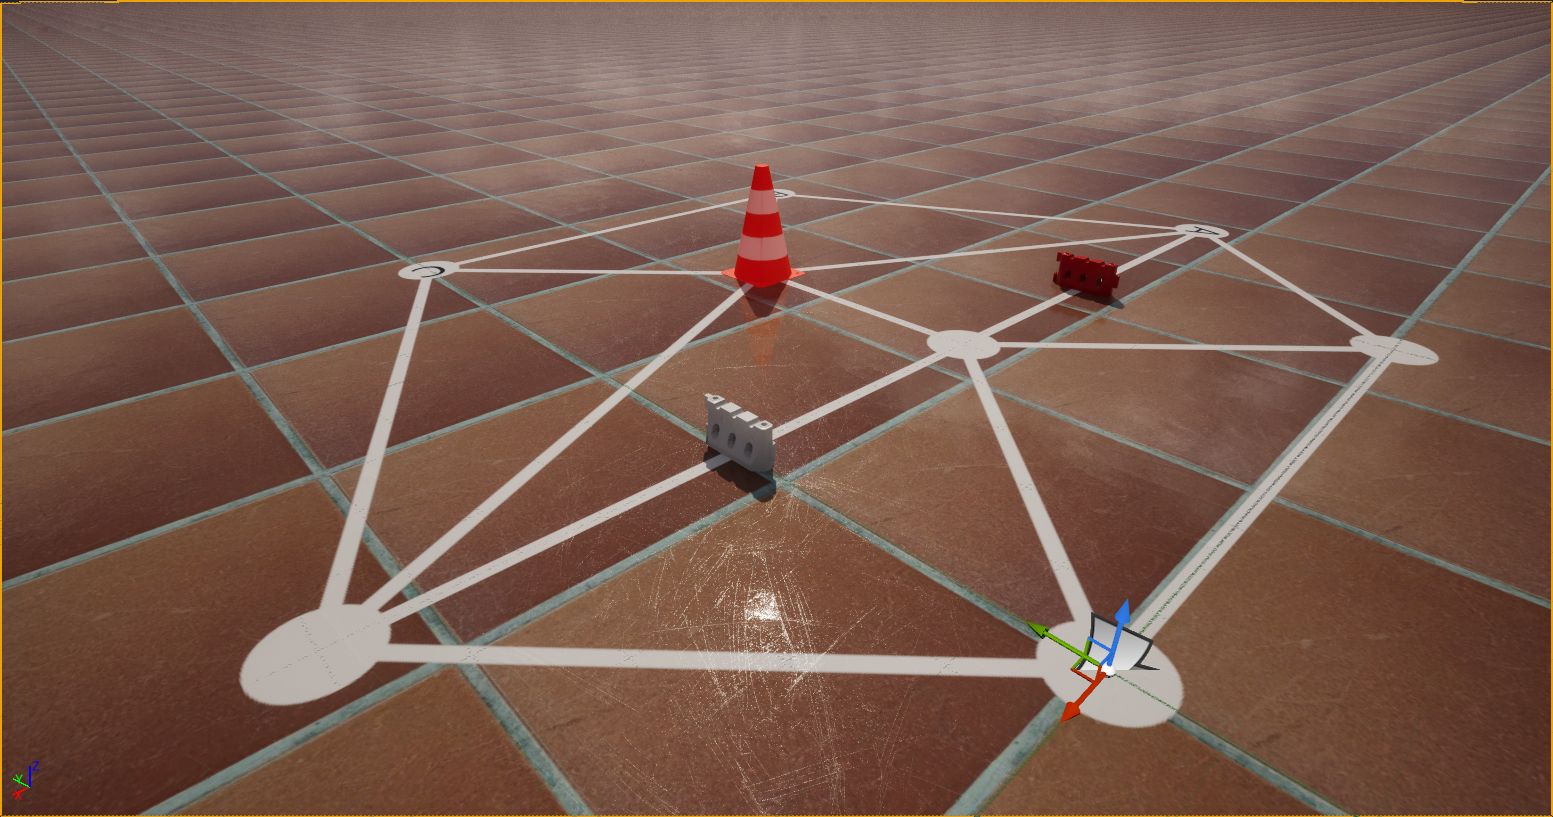
\includegraphics[width=0.9\textwidth]{img/unrealengine/overview.png}
            \caption{Übersicht Unreal Engine}
        \label{img:Übersicht Unreal Engine}
        \end{figure}
\subsection{Kamera-Konfiguration}
Unreal Engine erlaubt das einfache Testen von verschiedenen Kamera-Konfigurationen. Unter anderem Das Kamera-Sichtfeld, sowie verschiedene Neigungswinkel. In folgender Tabelle sind die Ergebnisse unterschiedlicher Kamerakonfigurationen zu sehen. Dabei stellt der grüne Kreis eine horizontale Distanz von 4.5m von der Kamera entfernt, und der weisse Kreis eine horizontale Distanz von 2m von der Kamera entfernt dar.
\begin{table}[h!]
    \centering
    \begin{tabular}{|c|c|c|c|}
        \hline
        & Höhe 30cm & Höhe 50cm & Höhe 75cm \\
        \hline
        \parbox[c][2cm][c]{4cm}{\centering Kamera FoV 75°, \\ Kameraneigung 30°} & 
        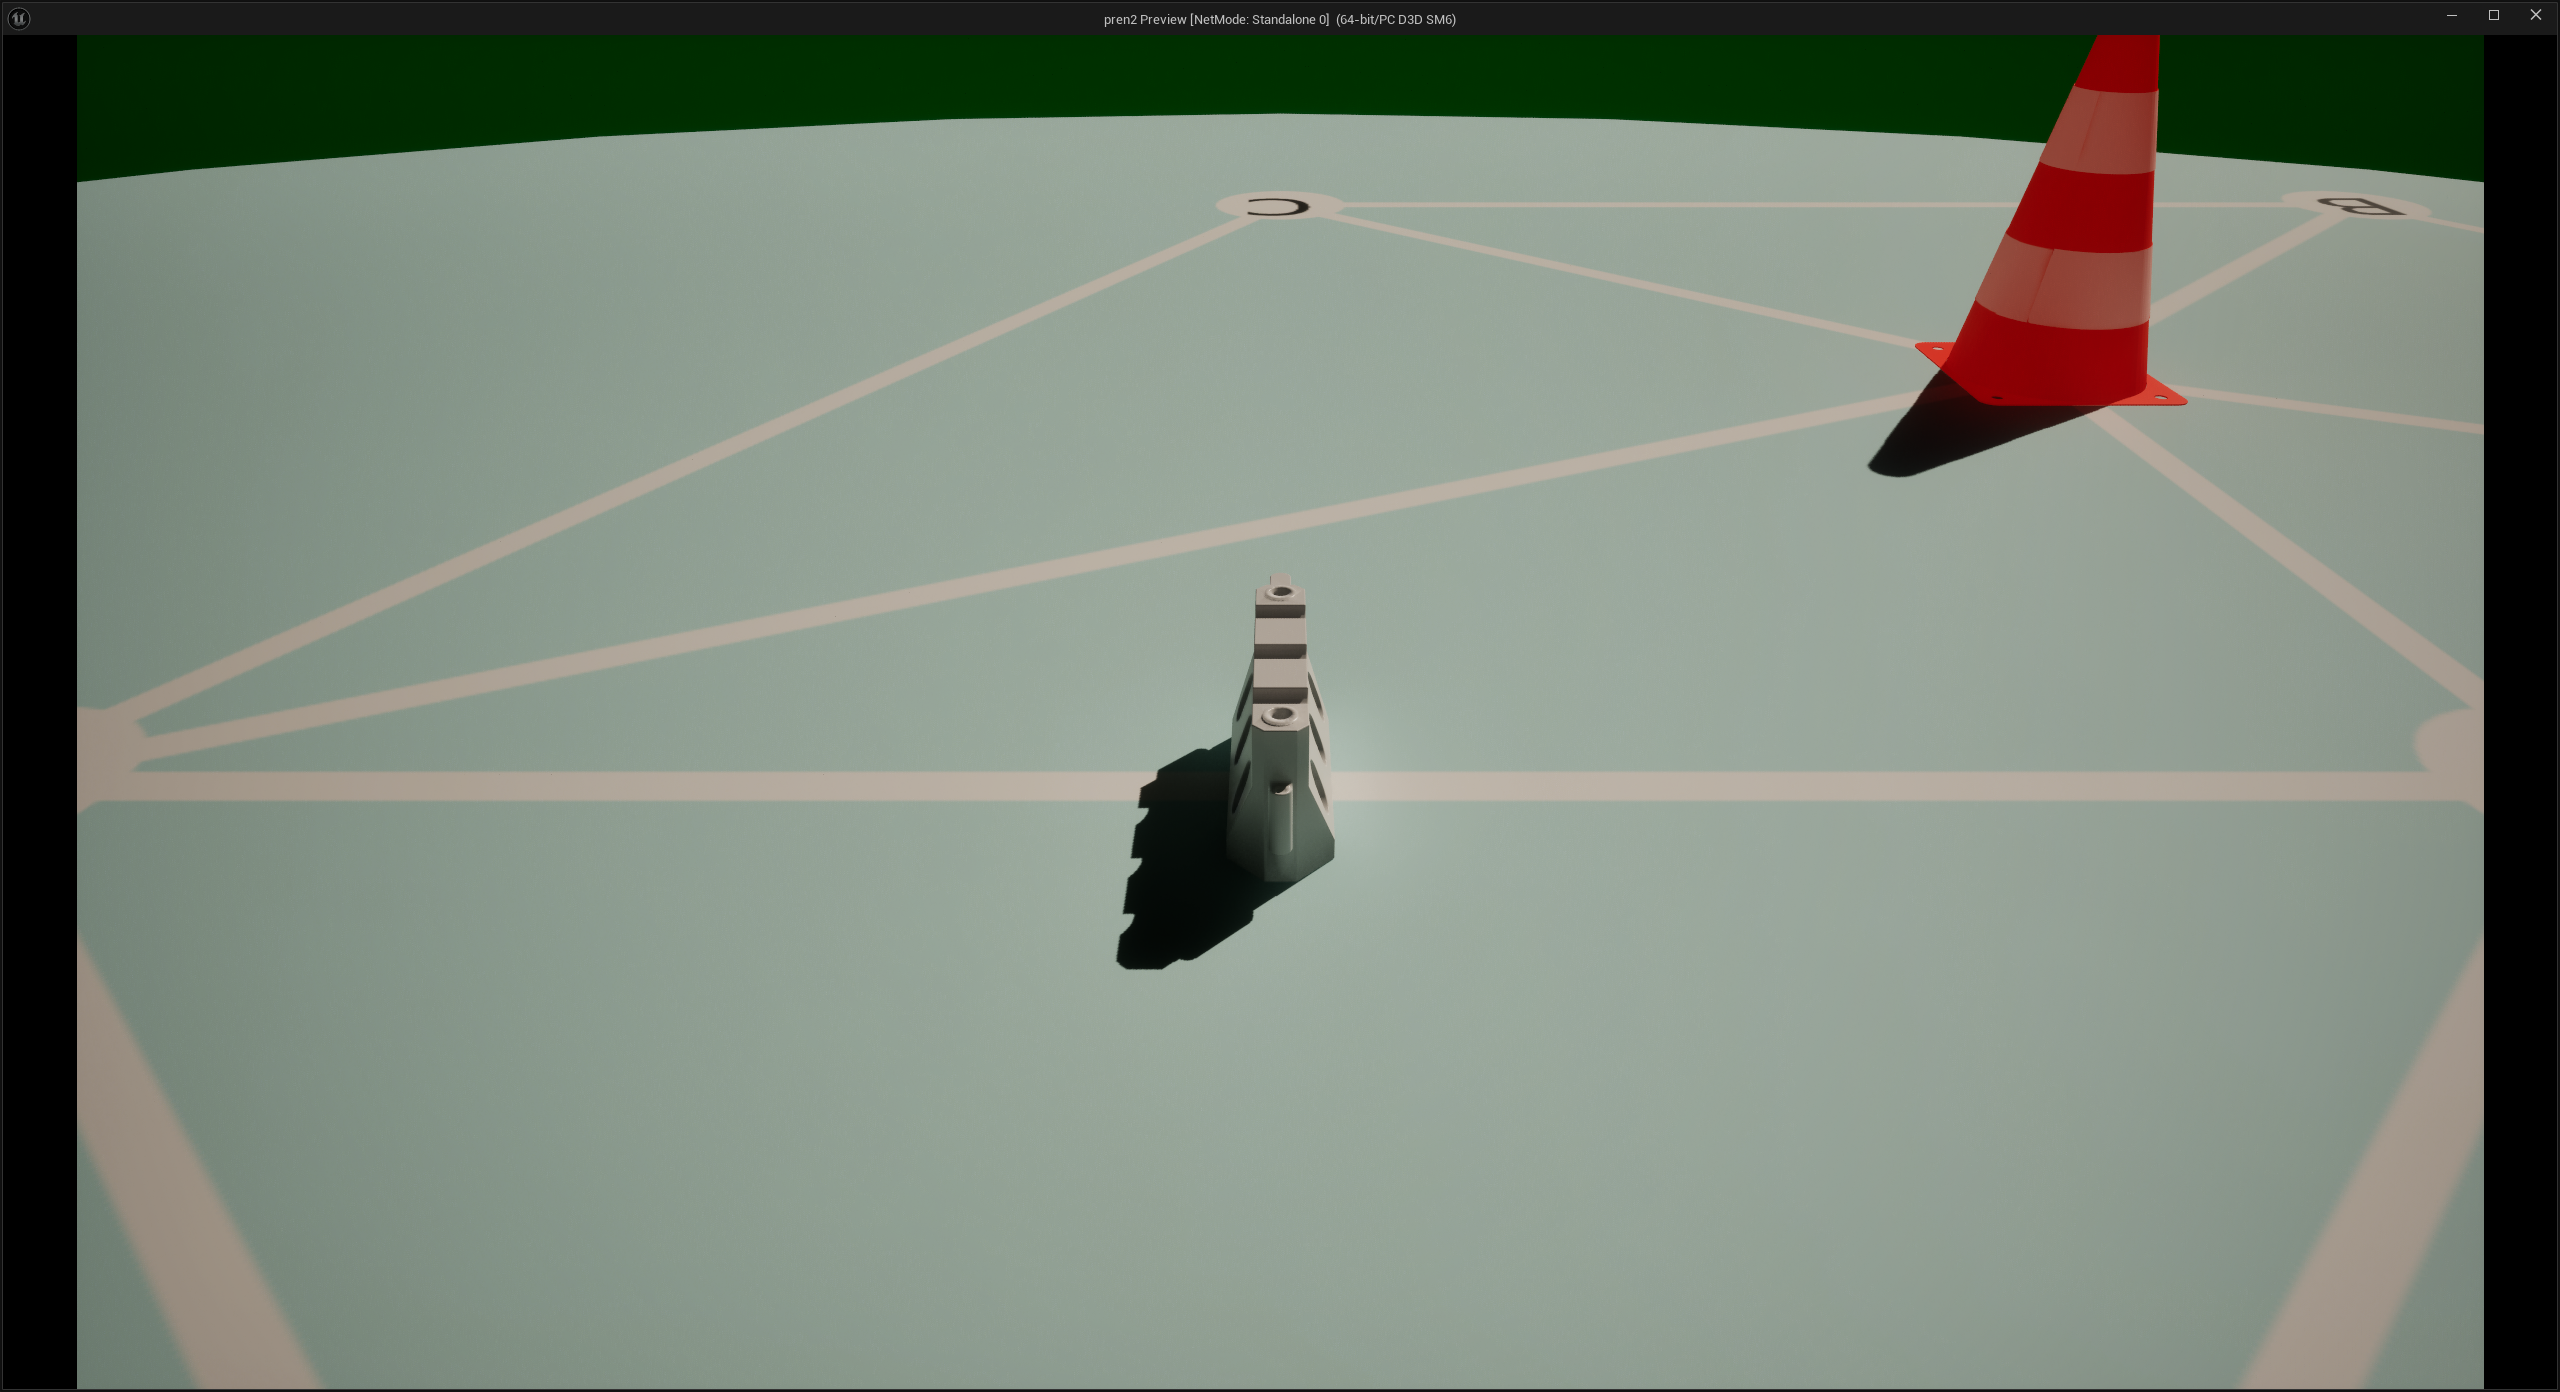
\includegraphics[width=4cm]{img/unrealengine/h30_f75_w30.png} & 
        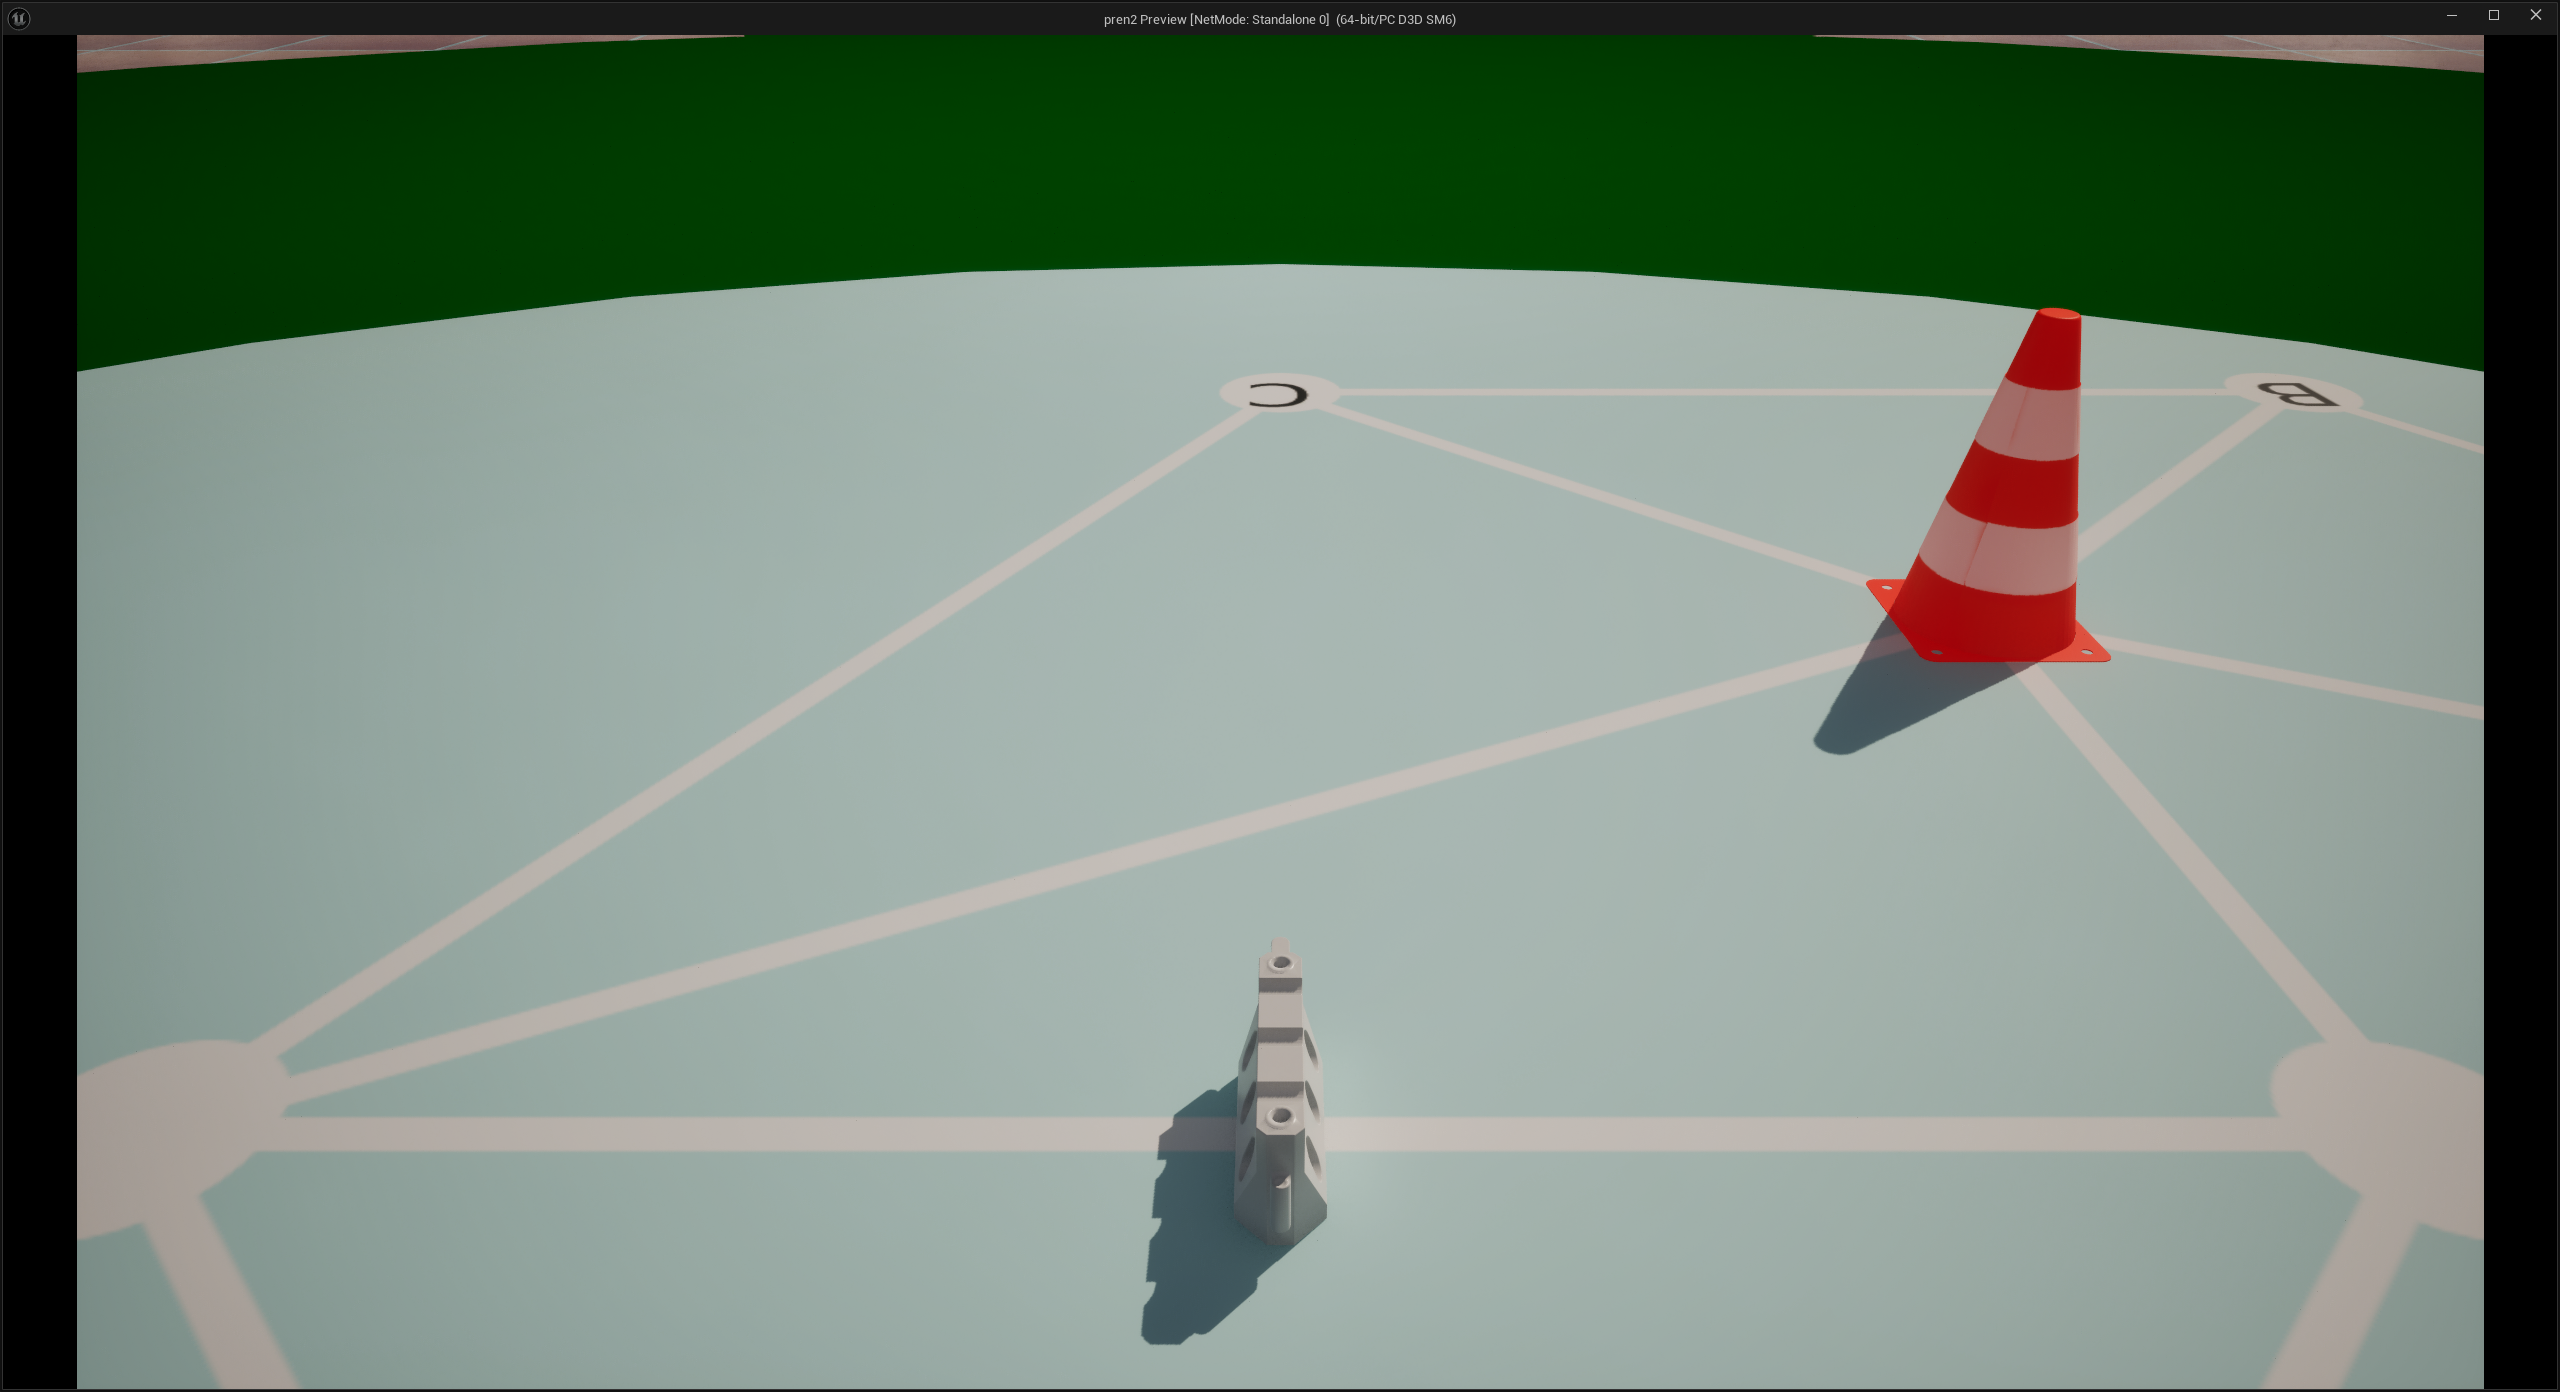
\includegraphics[width=4cm]{img/unrealengine/h50_f75_w30.png} & 
        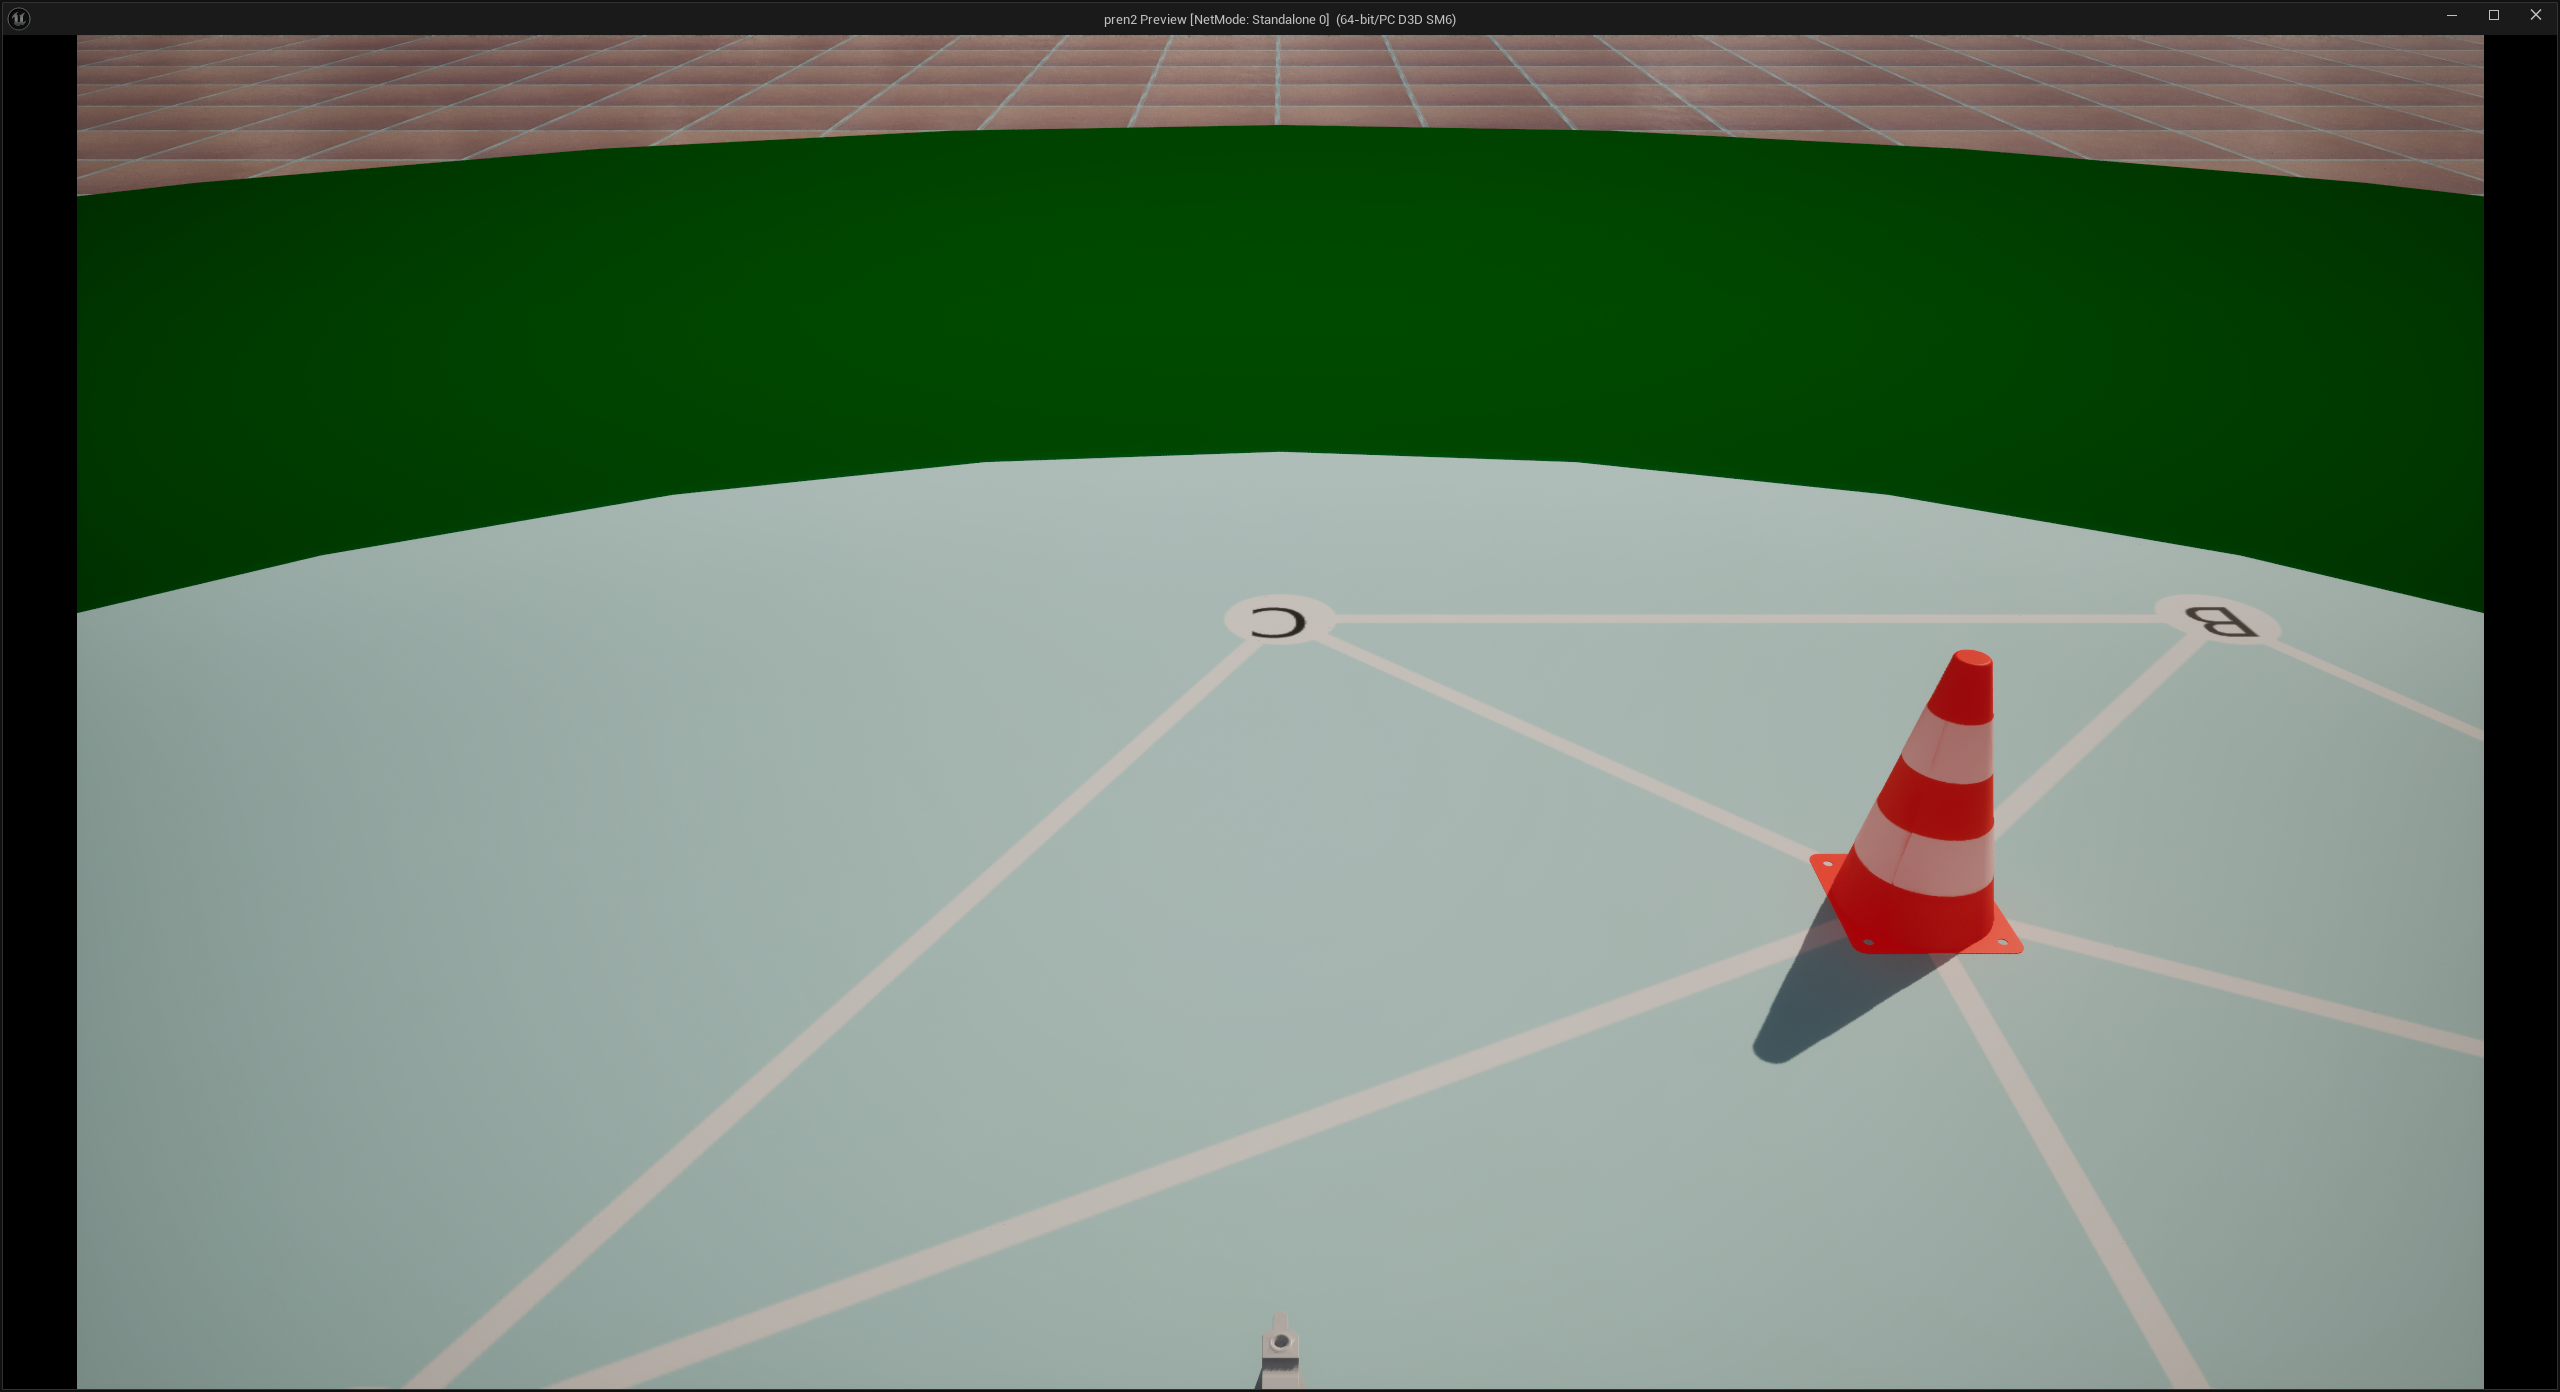
\includegraphics[width=4cm]{img/unrealengine/h75_f75_w30.png} \\
        \hline
        \parbox[c][2cm][c]{4cm}{\centering Kamera FoV 120°, \\ Kameraneigung 45°} & 
        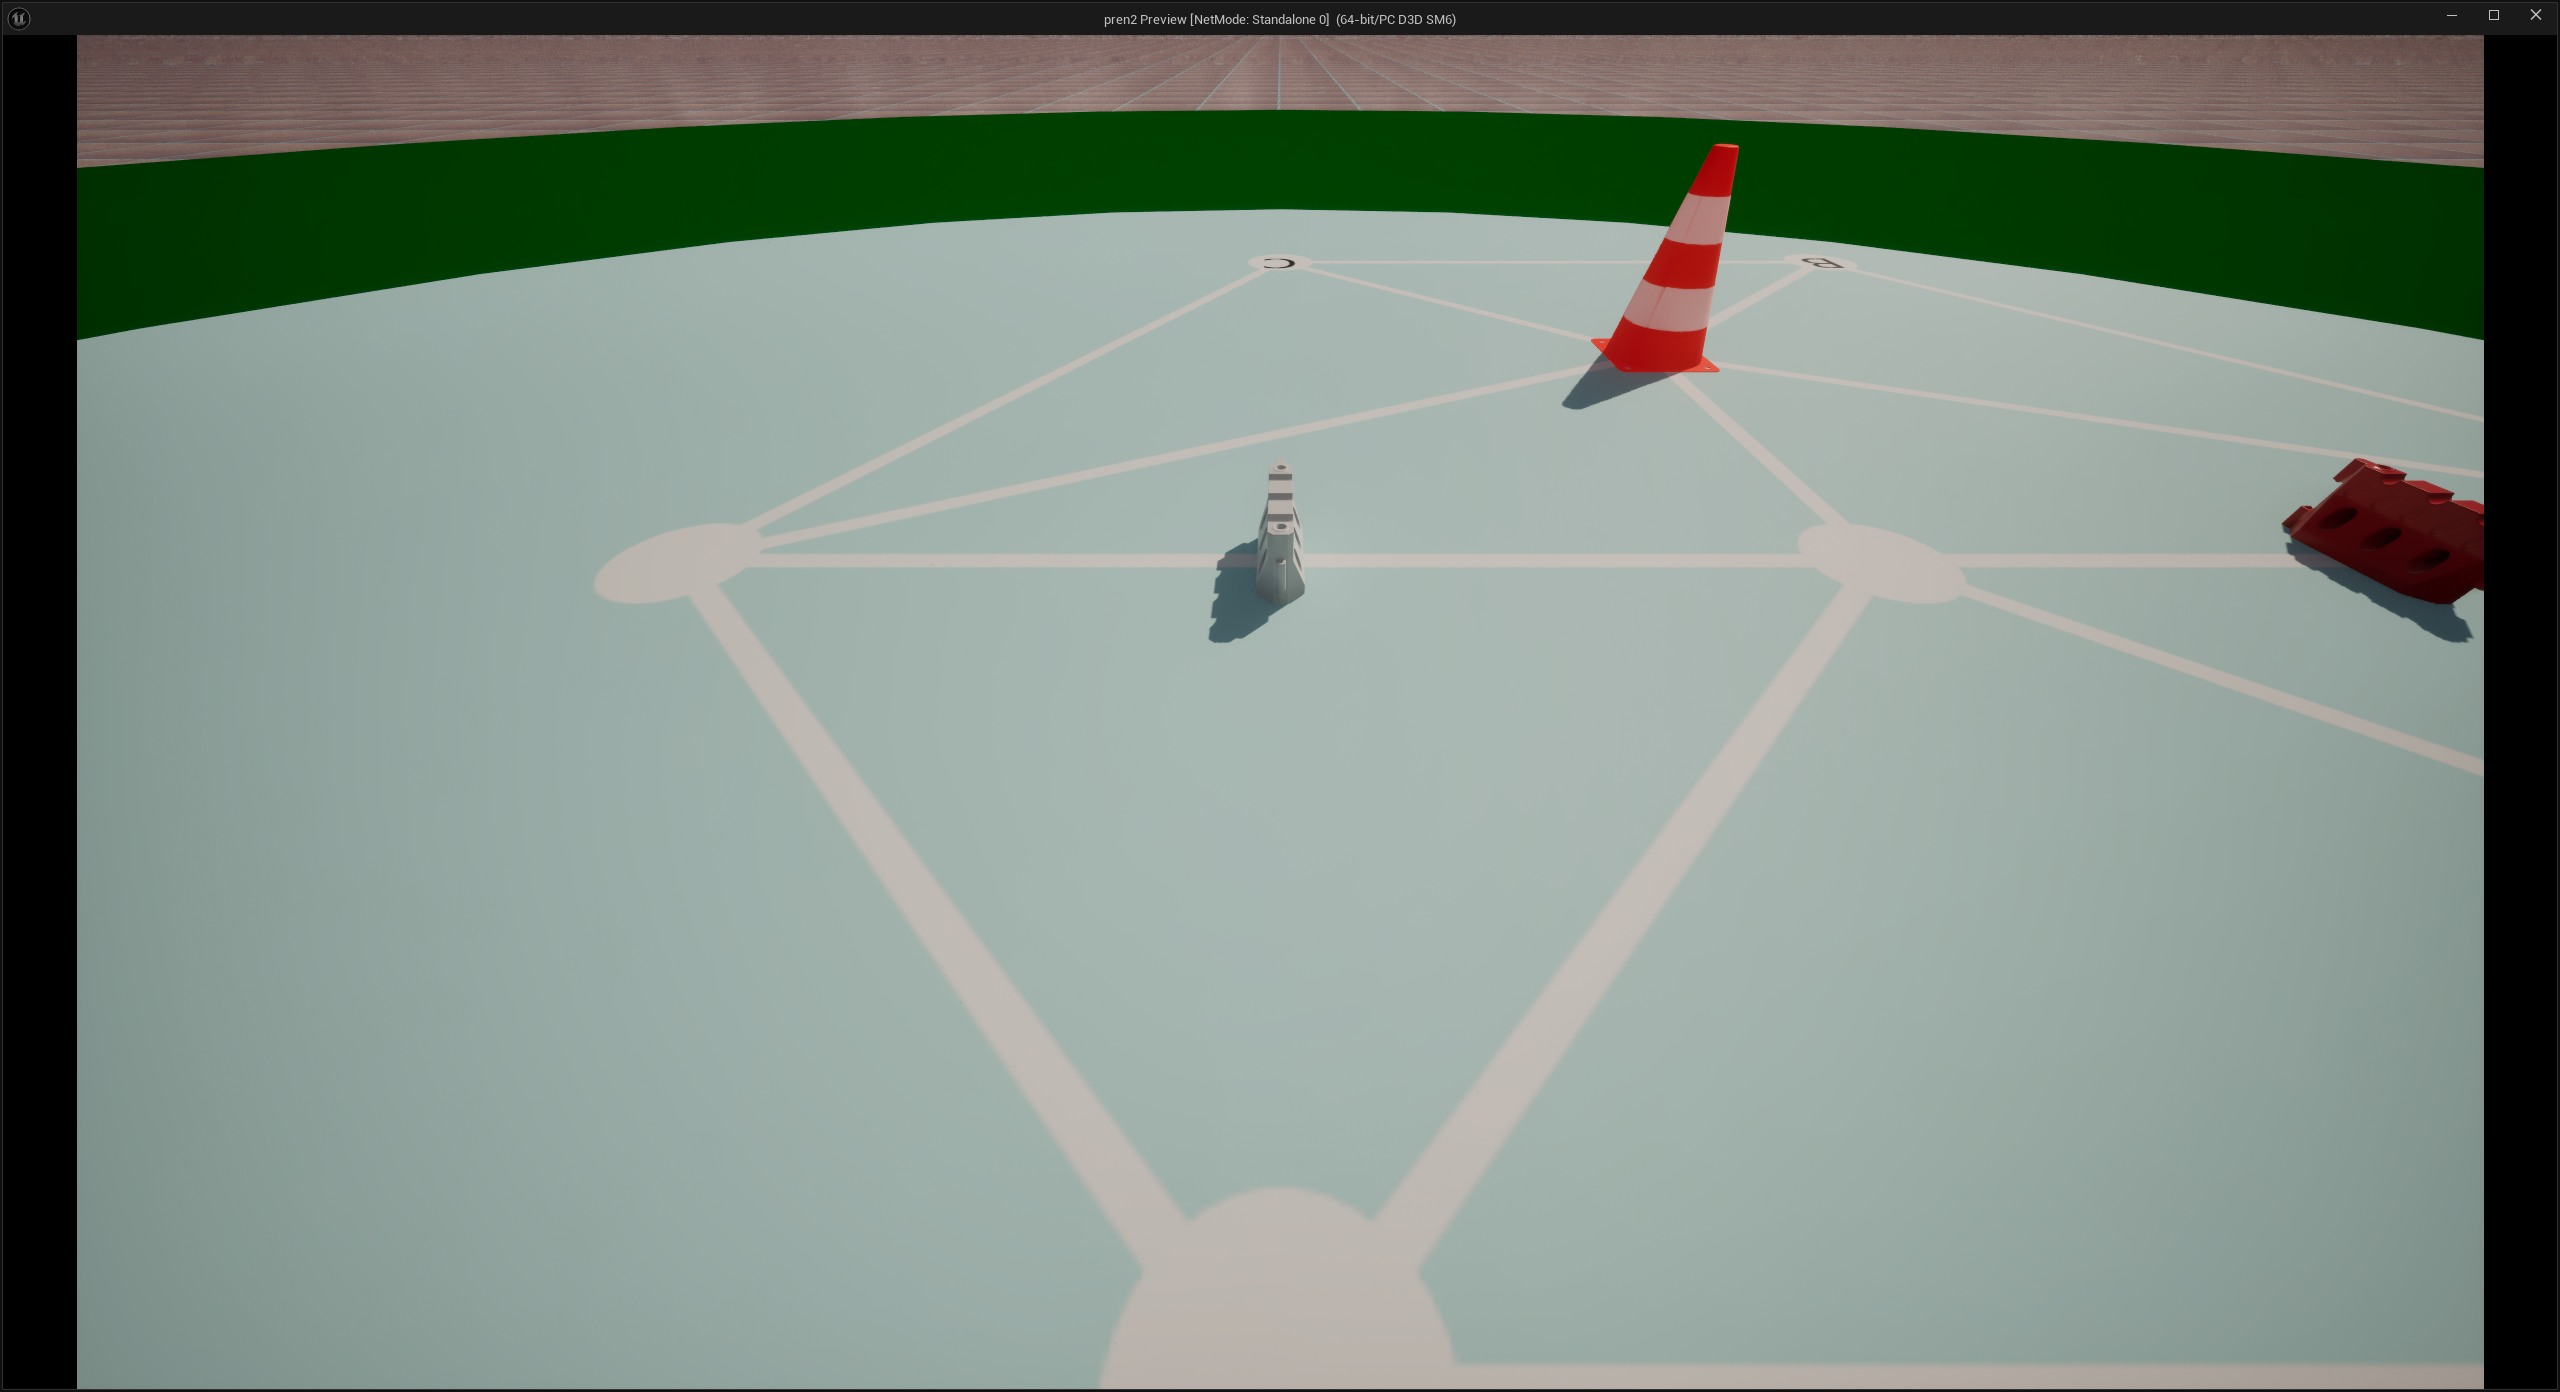
\includegraphics[width=4cm]{img/unrealengine/h30_f120_w45.png} & 
        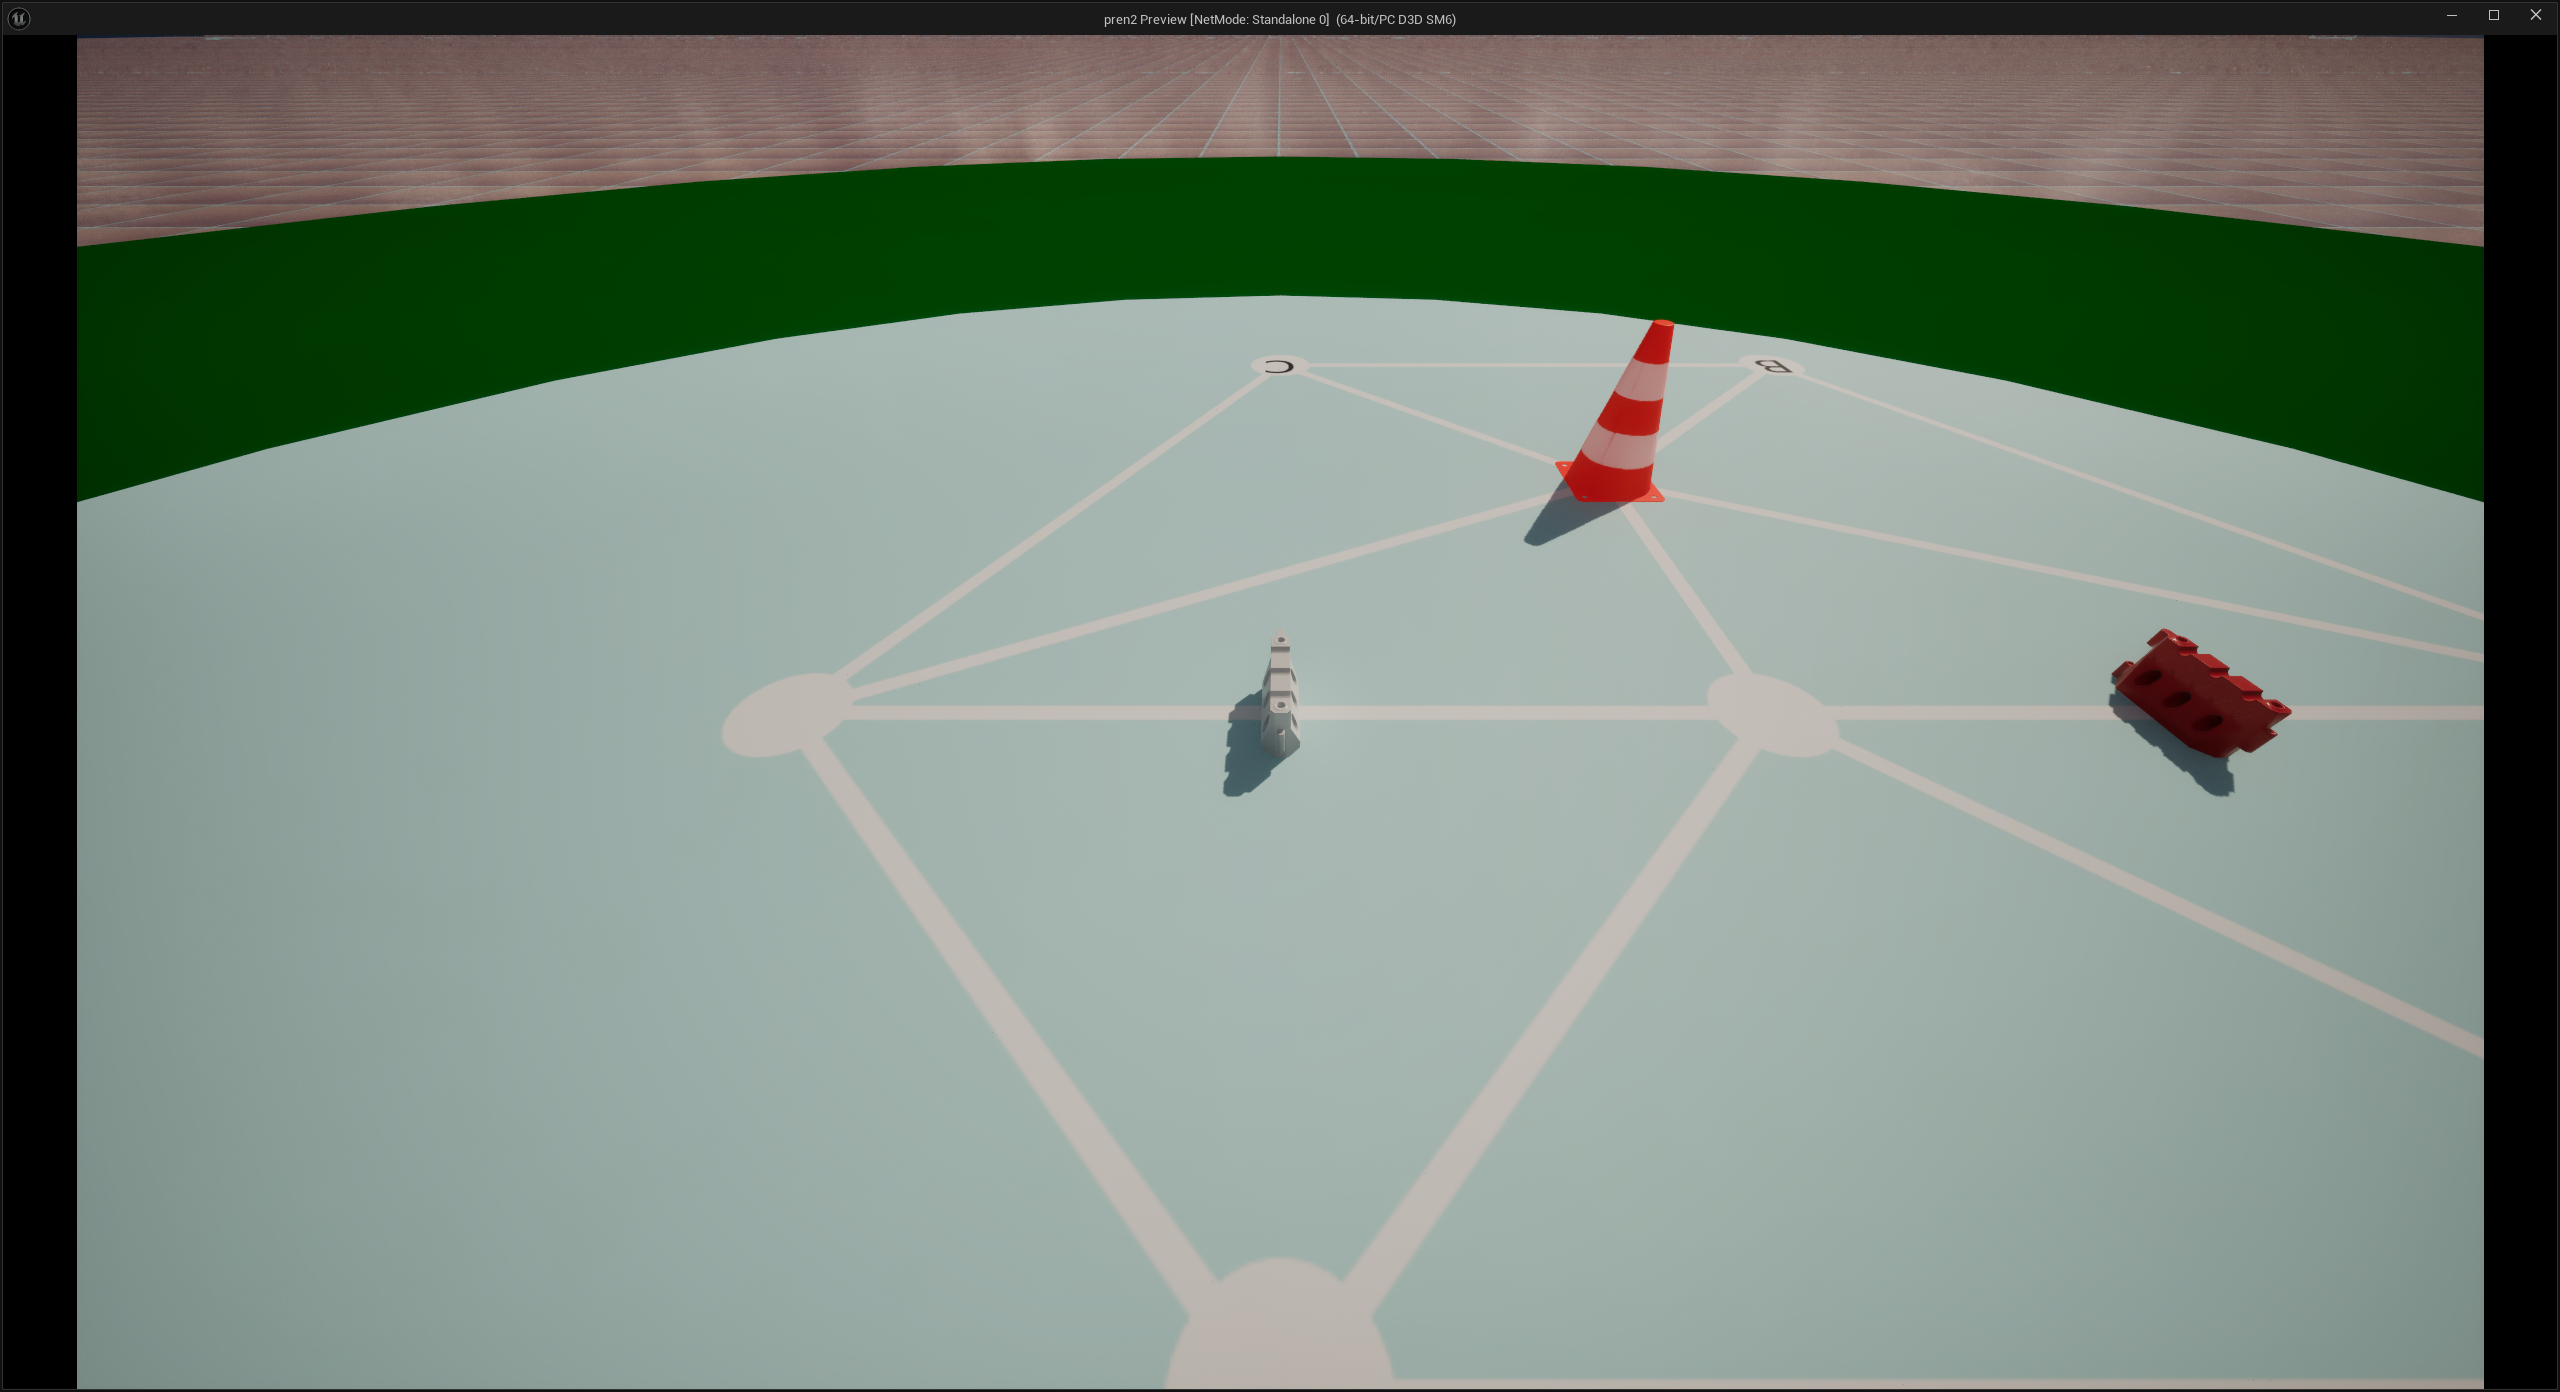
\includegraphics[width=4cm]{img/unrealengine/h50_f120_w45.png} & 
        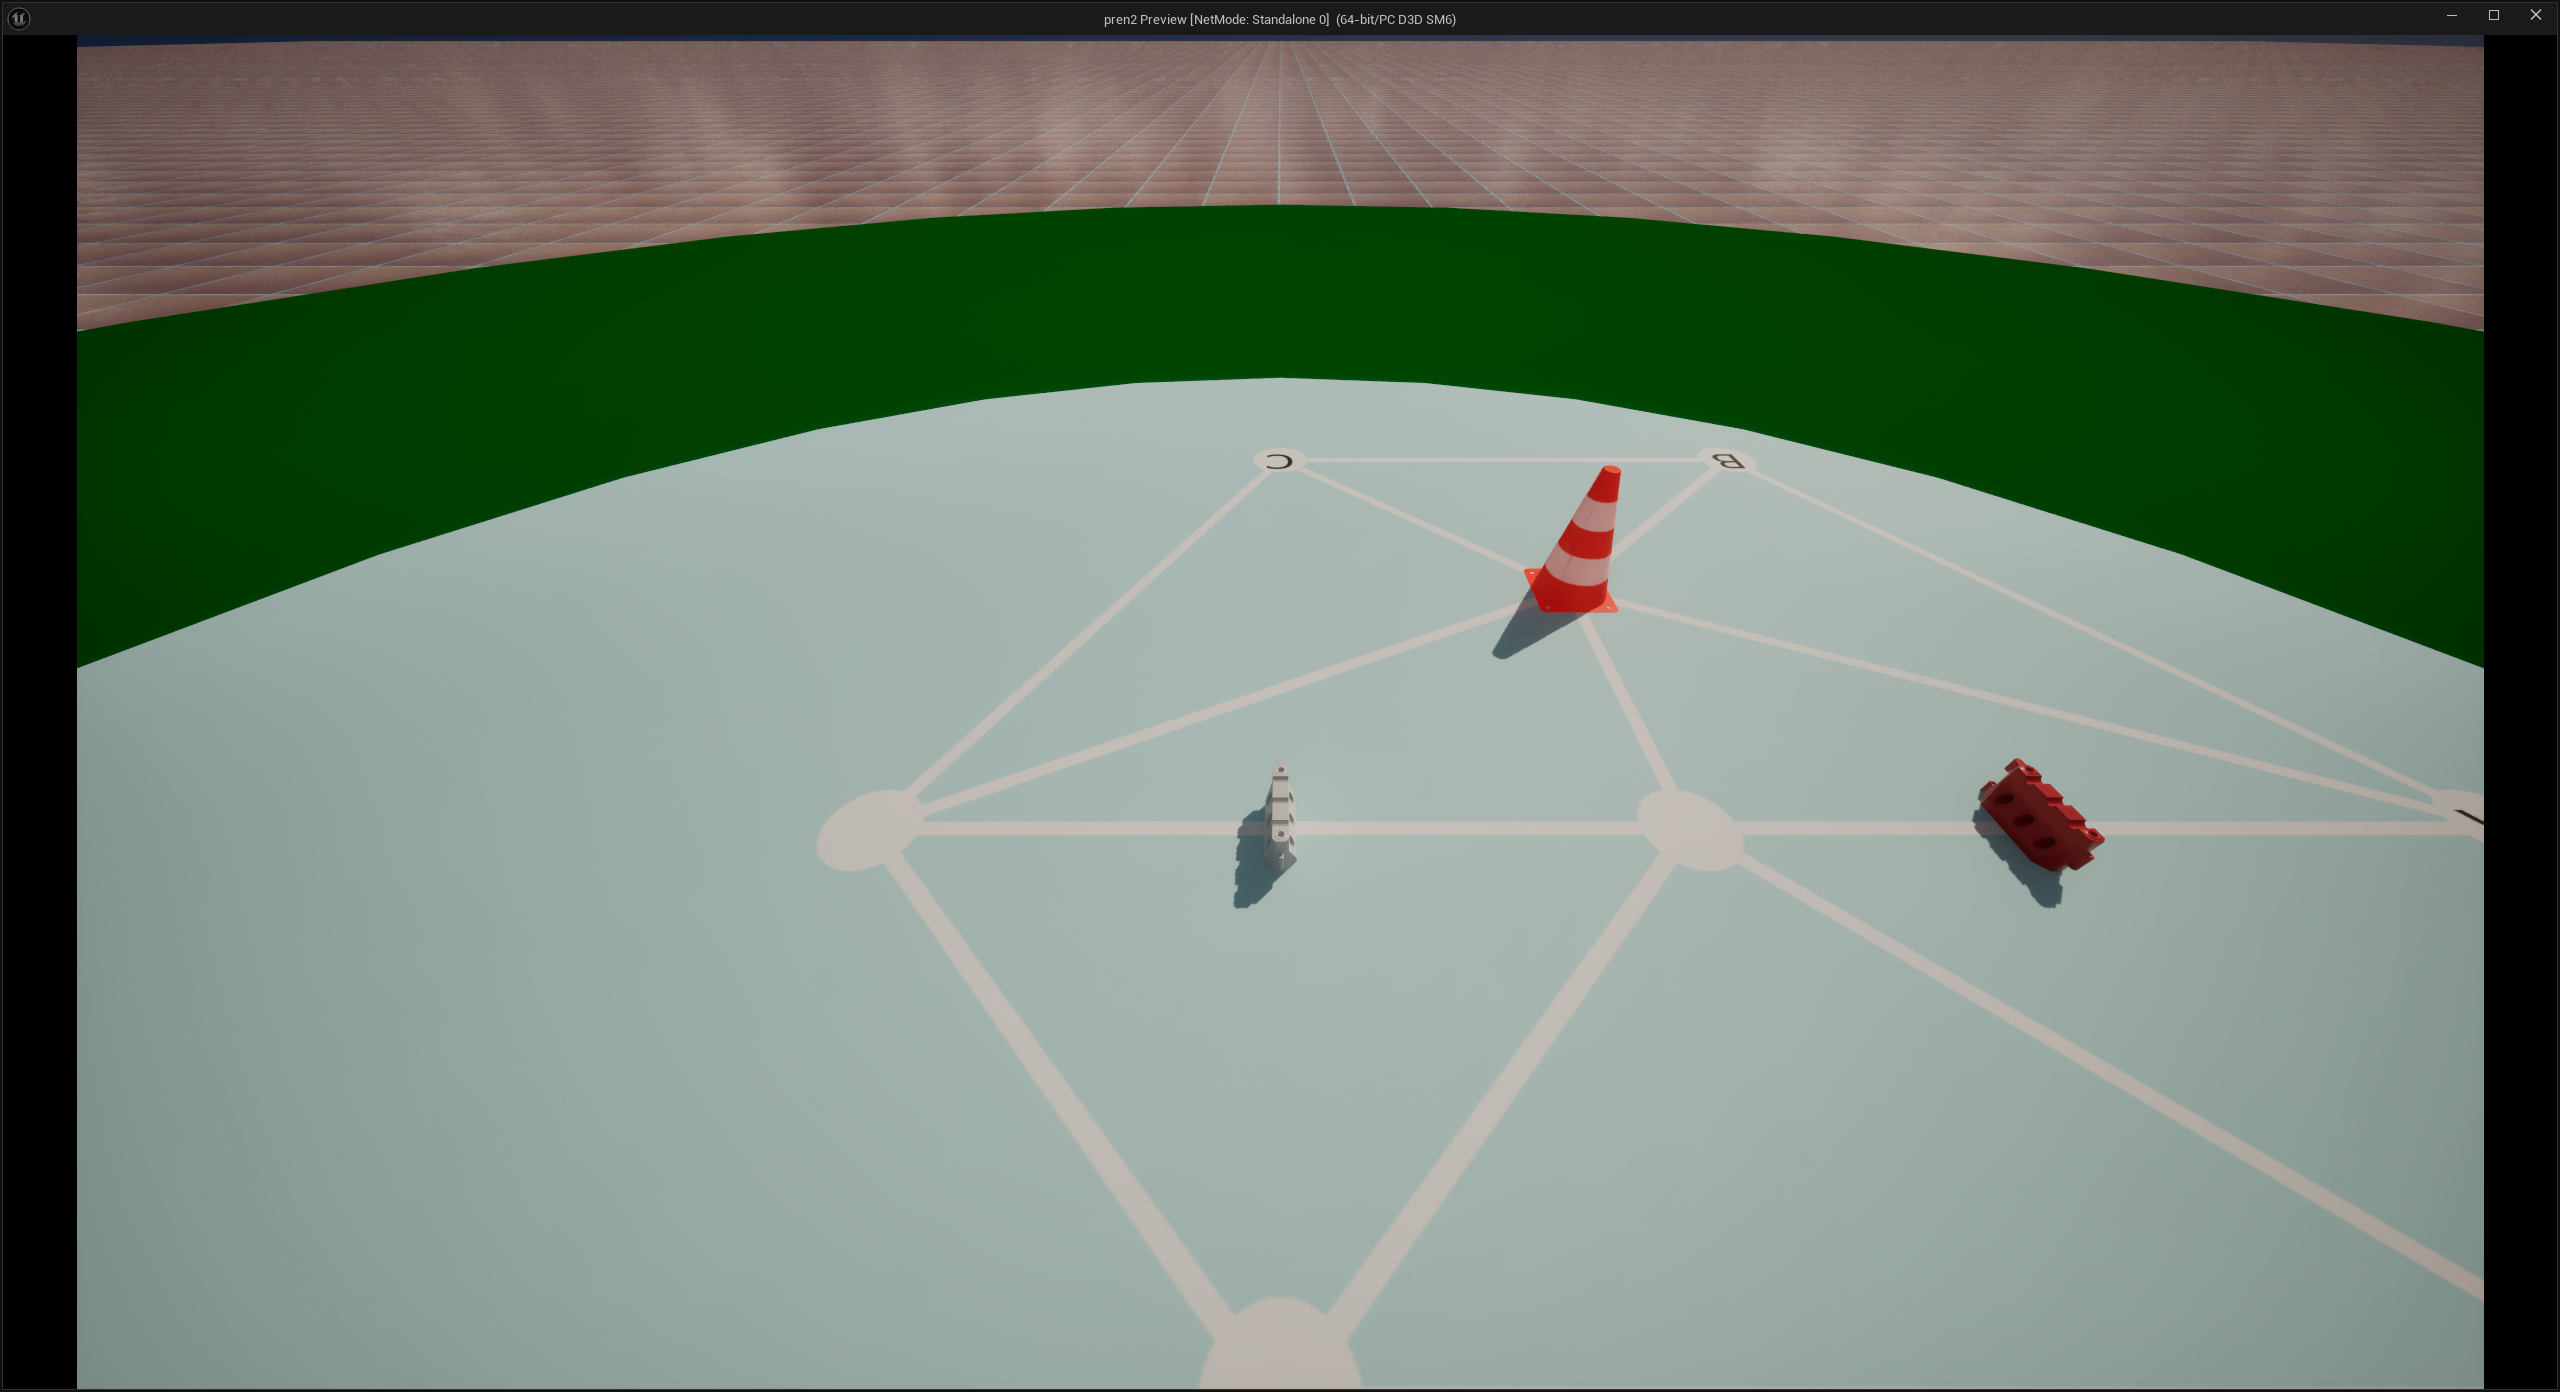
\includegraphics[width=4cm]{img/unrealengine/h75_f120_w45.png} \\
        \hline
    \end{tabular}
    \caption{Vergleich unterschiedlicher Kamera-Einstellungen und Höhen}
\end{table}


